\documentclass[main]{subfiles}


\title[AutoML: Introduction]{AutoML Motivation}
\subtitle{Success Stories of AutoML}
\author[Marius Lindauer]{Marius Lindauer}
\date{}

\titlebackground*{images/AutoML_HPO_2_2}

%\institute{}
%\date{}

\begin{document}
	
	\maketitle
	

%----------------------------------------------------------------------
%----------------------------------------------------------------------
\begin{frame}[c]{ChaLearn Automatic Machine Learning Challenge\\ \liturl{Guyon et al. 2019}{https://link.springer.com/chapter/10.1007/978-3-030-05318-5_10}}

\begin{columns}

\column{0.3\textwidth}


\includegraphics[width=1.0\textwidth]{images/chalearn}

\column{0.7\textwidth}

\begin{itemize}
    \item First full automatic AutoML competition
    \item Public leaderboard to test the AutoML system on datasets with given characteristics
    \item Code submission that needed to run under limited resources without human intervention
    \item In the first phase of the competition (2015), human teams also participated -- AutoML systems performed reasonably good already
    \item Key to win: Bayesian Optimization on a full pipeline + Ensembling (+ later: multi-fidelity optimization)
\end{itemize}

\end{columns}

\end{frame}
%-----------------------------------------------------------------------
%----------------------------------------------------------------------
\begin{frame}[c]{Gartner AI Hype Cycle 2019\\ \liturl{Gartner et al. 2019}{https://www.gartner.com/smarterwithgartner/top-trends-on-the-gartner-hype-cycle-for-artificial-intelligence-2019}}


\centering
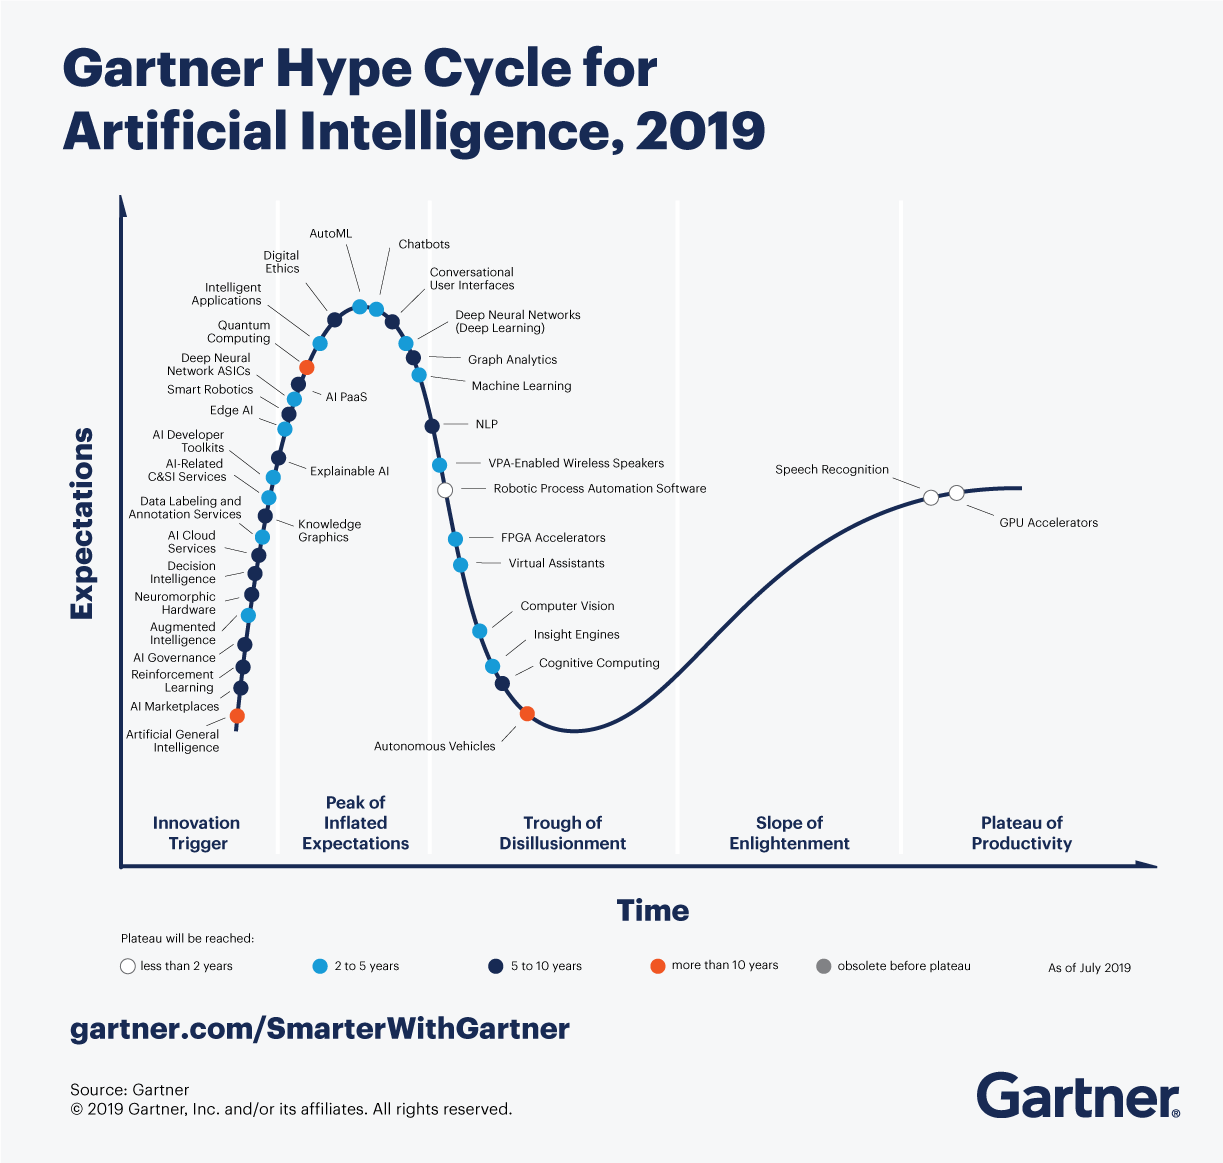
\includegraphics[width=0.57\textwidth]{images/automl_gartner.png}

\end{frame}
%-----------------------------------------------------------------------

%----------------------------------------------------------------------
\begin{frame}[c]{Black-Box Optimization Challenge at NeurIPS'20\\ \liturl{Turner et al. 2020}{https://proceedings.mlr.press/v133/turner21a.html}}

\begin{columns}

\column{0.3\textwidth}


\includegraphics[width=1.0\textwidth]{images/bbo}

\column{0.7\textwidth}

\begin{itemize}
    \item Very diverse set of black-box problems for machine learning $\leadsto$ typically hyperparameter optimization
    \item Although many developers still used grid or random search, the competition showed consistent results that more advanced methods performed better (e.g., Bayesian Optimization)
    \item However, given the diverse set of benchmarks, there was no clear single best approach
\end{itemize}

\end{columns}

\end{frame}
%-----------------------------------------------------------------------
%----------------------------------------------------------------------
\begin{frame}[c]{Using AutoML to Optimize Shape Error Prediction in Milling Processes \liturl{Denkena et al. 2020}{https://papers.ssrn.com/sol3/papers.cfm?abstract_id=3724234}}

\begin{columns}

\column{0.4\textwidth}


\includegraphics[width=
1.0\textwidth]{01_AutoML/images/milling_process.png}

\column{0.6\textwidth}

\centering

\includegraphics[width=0.65\textwidth]{01_AutoML/images/automl_milling.png}


\end{columns}

\end{frame}
%-----------------------------------------------------------------------
%TODO
%----------------------------------------------------------------------
\begin{frame}[c]{2024 AutoML Grand Prix\\ \liturl{Kaggle}{https://www.kaggle.com/automl-grand-prix}}

\begin{columns}

\column{0.3\textwidth}

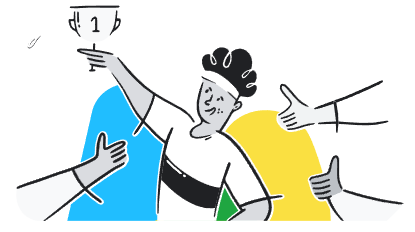
\includegraphics[width=1.0\textwidth]{images/automl_grand_prix.png}

\column{0.7\textwidth}

\begin{itemize}
    \item Each month, one new task for five months
    \item Only 24h to participate -- humans got more time!
    \item Winner of each competition got $25$ points (also among human teams) -- best AutoML system got $73$ points out of $125$ points
    \item Winner: LightAutoML~\liturl{Vakhrushev et al}{https://arxiv.org/pdf/2109.01528}
    \begin{itemize}
        \item \alert{Note}: Preprocessing of the data turned out to be a major factor
    \end{itemize}
    
\end{itemize}

\end{columns}

\end{frame}
%-----------------------------------------------------------------------
%----------------------------------------------------------------------
\begin{frame}[c]{AutoML is Actively Being Used by Companies\\ \liturl{Dilmegani 2025}{https://research.aimultiple.com/automl-case-studies/}}

\centering
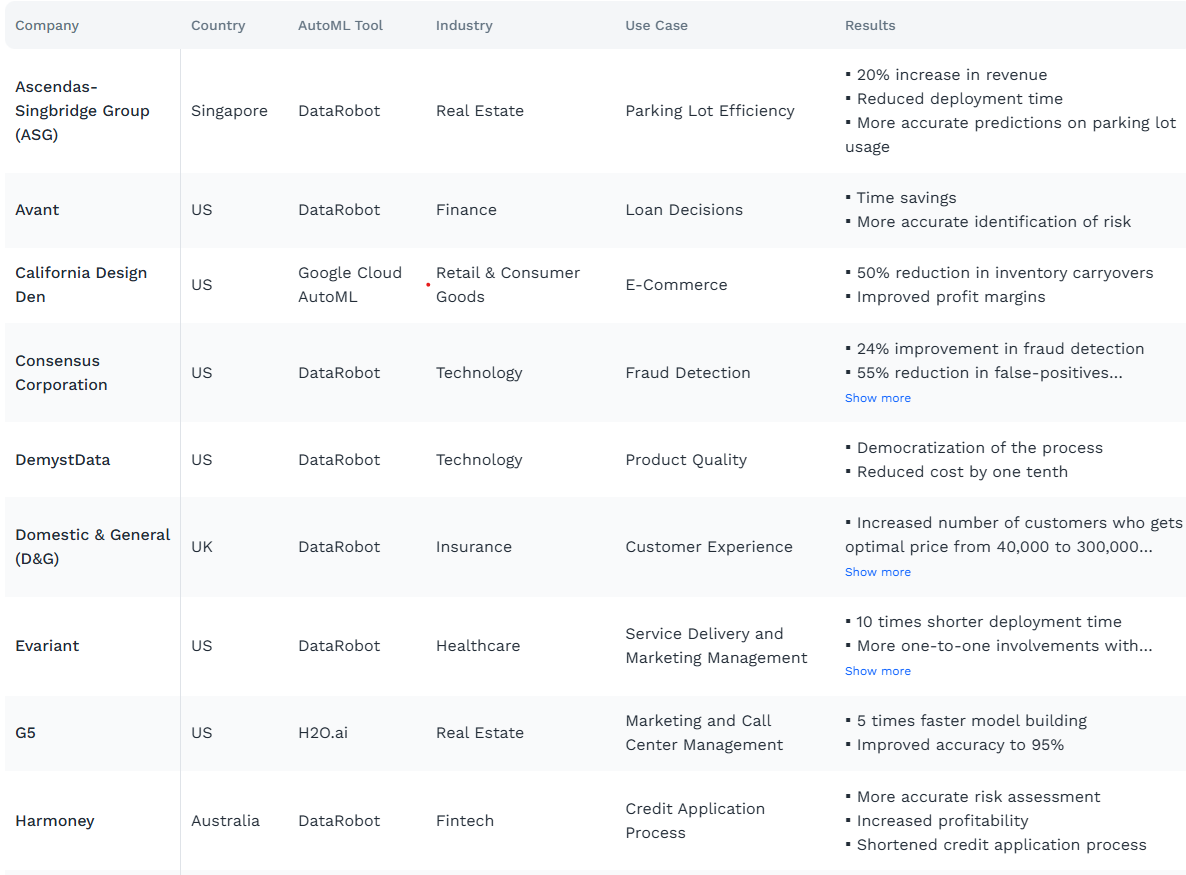
\includegraphics[width=.7\textwidth, trim={0 200px 0 0}, clip]{images/success_automl.png}

Disclaimer: We were not able to verify all of these since no sources were given.

\end{frame}
%-----------------------------------------------------------------------
%----------------------------------------------------------------------
\begin{frame}[c]{The AutoML Community}

\begin{itemize}
    \item Annual international conference on AutoML since 2021: \url{https://www.automl.cc}
    \item Monthly, online AutoML Seminar: \url{https://automl-seminars.github.io}
    \item AutoML Podcast: \url{https://automlpodcast.com}
    \item Many AutoML packages (AutoGluon and Optuna probably the most famous ones as of Summer 2025), see \url{https://automl.space}
    \item An AutoML MOOC \ldots
\end{itemize}

\end{frame}
%-----------------------------------------------------------------------

%----------------------------------------------------------------------
\begin{frame}{Summary} 

Most important insights from this video:

\begin{enumerate}
    \item Although the first ideas on AutoML go back to the 70s with algorithm selection~\liturl{Rice 1976}{https://www.sciencedirect.com/science/chapter/bookseries/abs/pii/S0065245808605203} and 90s with neuro-evolution~\liturl{Maniezzo 1994}{https://ieeexplore.ieee.org/document/265959/}, the breakthrough started around 2012-2015 as an implicit consequence of the Deep learning hype
    \item AutoML showed impressive results on many domains; most impressive results still on tabular data
    \item AutoML can perform as well as top human teams (in pre-defined settings)
    \item AutoML is already actively being used by many companies
\end{enumerate}


\end{frame}

\end{document}
